% SPDX-License-Identifier: CC-BY-SA-4.0
% Author: Matthieu Perrin
% Part: Introduction
% Section: Words and languages
% Exercise: Words

\begingroup

\begin{exercice}[Le problème \textsc{Ensemble Stable}]

  Étant donné un graphe $G$, un {\em ensemble stable} de $G$ est un ensemble de sommets deux à deux non adjacents dans $G$.
  Autrement dit, pour toute paire $u, v$ de sommets de cet ensemble, l'arête $\langle u, v\rangle$ {\em n'existe pas} dans $G$.

  Par exemple, dans le graphe ci-dessous, les sommets $1, 4, 5$ et $6$ forment un ensemble stable.

  \begin{center}
    \begin{tikzpicture}[x=10mm, y=10mm]
      \node[graph node, circle] (1) at (1,2) {1};
      \node[graph node, circle] (2) at (3,2) {2};
      \node[graph node, circle] (3) at (0,1) {3};
      \node[graph node, circle] (4) at (2,1) {4};
      \node[graph node, circle] (5) at (4,1) {5};
      \node[graph node, circle] (6) at (1,0) {6};
      \node[graph node, circle] (7) at (3,0) {7};

      \draw[thick] (3) -- (1) -- (2) -- (5) -- (7) -- (6) -- (3);
      \draw[thick] (3) -- (2) -- (4) -- (7) -- (3);
    \end{tikzpicture}
  \end{center}

  On s'intéresse au problème de décision \textsc{Ensemble Stable}:

  \Probleme{Ensemble Stable}{
    Une paire $\langle G, k \rangle$ formée d'un graphe non orienté $G=\langle V, E\rangle$ et d'un entier $k$.
  }{
    Existe-t-il un ensemble stable de taille au moins $k$ dans $G$ ?
  }

  Le but de cet exercice est de montrer qu'\textsc{Ensemble Stable} est NP-complet.
  
  \begin{question}
  \item\label{ex3.Q8} Expliquez pourquoi le problème \textsc{Ensemble Stable} appartient à la classe NP.
    Pour cela, précisez quel certificat fournir pour une réponse ``oui'', et expliquez comment vérifier ce certificat en temps polynomial.
  \end{question}
  \begin{correction}
    Un certificat pour le problème \textsc{Ensemble Stable} est un tableau $T$ de $k$ sommets. Si l'instance est positive, on a forcément $k \le |E| \le |G|$.
    
    Pour vérifier ce certificat (qu'on suppose déjà parsé sous la forme d'un tableau), il faut
    \begin{itemize}
    \item vérifier que la longueur est bien $k$, en $\mathcal{O}(1)$; 
    \item vérifier que tous les éléments du tableau sont bien des éléments de $E$, en $\mathcal{O}(k)$; 
    \item pour chaque paire d'indices $0 \le i, j < k$, vérifier que $T[i] \neq T[j]$ et que $\langle i, j \rangle \notin E$.
      Il y a $\mathcal{O}(k^2)$ paires d'indices, et suivant l'encodage du graphe, chaque tour de boucle peut coûter jusqu'à  $\mathcal{O}(|G|)$. 
    \end{itemize}
    Finalement, vérifier le certificat est bien polynômial en la taille du graphe. 
  \end{correction}

  On souhaite maintenant démontrer que $\textsc{3-SAT} \leq_P \textsc{Ensemble Stable}$. On rappelle et précise la définition de \textsc{3-SAT}
  utilisée dans cet exercice. 

  \Probleme{3-SAT}{
    Une formule booléenne $\varphi = C_1 \wedge C_2 \wedge \ldots \wedge C_p$,  
    où chaque clause $C_i$ ($1 \leq i \leq p$) est une disjonction d'\textbf{exactement} trois littéraux,
    et chaque littéral est soit une variable $x_j$, soit une négation $\lnot x_j$  
    pour une variable $x_j$ parmi un ensemble $\{x_1, x_2, \ldots, x_n\}$.
  }{
    Existe-t-il une valuation $\{x_1, x_2, \ldots, x_n\} \rightarrow \{\text{vrai}, \text{faux}\}$ qui satisfait $\varphi$ ?
  }

  Pour les premières questions de l'exercice, on considère l'instance $\psi$ particulière de \textsc{3-SAT} suivante : 
  $$\psi =
  \underbrace{(x_1 \vee x_2 \vee \neg x_3)}_{C_1}
  \wedge
  \underbrace{(\neg x_1 \vee \neg x_2 \vee \neg x_4)}_{C_2}
  \wedge
  \underbrace{(\neg x_2 \vee x_3 \vee \neg x_4)}_{C_3}
  \wedge
  \underbrace{(\neg x_1 \vee \neg x_2 \vee x_4)}_{C_4}
  $$
  
  \ifcorrection{\newpage}
  \begin{question}
  \item\label{ex3.Q1} Déterminez des valeurs pour les variables $x_1, x_2, x_3$ et $x_4$ qui satisfont $\psi$.
  \end{question}
  \begin{correction}
    Par exemple, $x_1 = x_3 = \text{vrai}$ et $x_2 = x_4 = \text{faux}$
  \end{correction}
  
  On définit maintenant une transformation $f$ qui, à chaque formule $\varphi$ de \textsc{3-SAT},
  associe une instance \linebreak $f(\varphi) = \langle G, k\rangle$ du problème \textsc{Ensemble Stable} construite selon les règles suivantes :
  \begin{itemize}
  \item $k=p$ (le nombre de clauses de $\varphi$),
  \item le graphe $G$ est construit comme ceci.
    \begin{itemize}
    \item Pour chaque clause $C_i$, on ajoute un triangle dont chacun des 3 sommets aura pour nom ``$i:l$''
      formé de l'indice $i$ de la clause et d'un des littéraux $l$ de $C_i$.
      On appellera chaque triangle un ``\underline{triangle-clause}''.

      Par exemple, pour une clause $C_i=(x_2\vee \neg x_4 \vee x_5)$, on ajoute dans $G$:

      \begin{center}
        \begin{tikzpicture}[x=20mm, y=20mm]
          \node[graph node] (C) at (.5,0.866) {$i : x_2$};
          \node[graph node] (A) at (0,0) {$i : \lnot x_4$};
          \node[graph node] (B) at (1,0) {$i : x_5$};

          \draw[thick] (A) -- (B) -- (C) -- (A);
        \end{tikzpicture}
      \end{center}

    \item On relie chaque paire de sommets représentant des littéraux opposés ($i : x_m$ et $j : \neg x_m$) par une arête.

      Par exemple, pour deux clauses $C_i=(x_2\vee \neg x_4 \vee x_5)$ et $C_j=(\neg x_2\vee \neg x_4 \vee \neg x_5)$ de $\varphi$, on a la configuration suivante dans $G$:

      \begin{center}
        \begin{tikzpicture}[x=20mm, y=20mm]
          % Triangle i
          \node[graph node] (C) at (.5,0.866) {$i : x_2$};
          \node[graph node] (A) at (0,0)      {$i : \lnot x_4$};
          \node[graph node] (B) at (1,0)      {$i : x_5$};

          \draw[thick] (A) -- (B) -- (C) -- (A);

          % Triangle j
          \node[graph node] (F) at (3.5,0.866) {$j : \lnot x_2$};
          \node[graph node] (D) at (3,0)       {$j : \lnot x_4$};
          \node[graph node] (E) at (4,0)       {$j : \lnot x_5$};

          \draw[thick] (D) -- (E) -- (F) -- (D);

          % Liens inter-triangles
          \draw[blue, thick] (C) -- (F);
          \draw[red, thick] (B) to[bend right=20] (E);
        \end{tikzpicture}
      \end{center}

      
    \end{itemize}
  \end{itemize}
  
  \begin{question}
  \item\label{ex3.Q2} Fournissez l'instance $f(\psi) = \langle G_\psi, k_\psi \rangle$ d'\textsc{Ensemble Stable}
    obtenue par la transformation de la formule $\psi$ utilisée dans la question~\ref{ex3.Q1} : pour cela, dessinez $G_\psi$ et donnez la valeur de $k_\psi$.
  \end{question}
  \begin{correction}

    $k=4$
    
    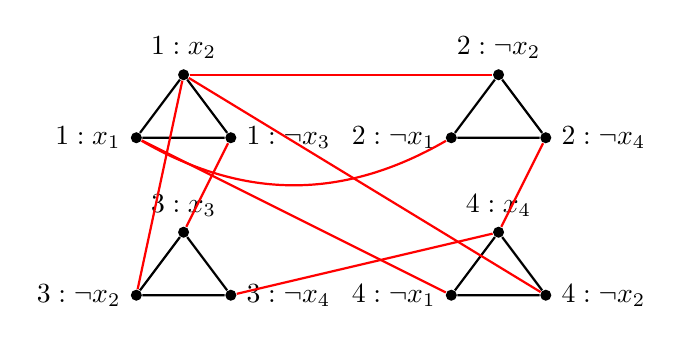
\begin{tikzpicture}[xscale=2,yscale=2]

      % Clause C1 : (x1 ∨ x2 ∨ ¬x3)
      \node[circle, fill, inner sep=0pt, minimum size=4pt, label=above:$1 : x_2$] (C1C) at (1,1.7) {};
      \node[circle, fill, inner sep=0pt, minimum size=4pt, label=left:$1 : x_1$] (C1A) at (0.7,1.3) {};
      \node[circle, fill, inner sep=0pt, minimum size=4pt, label=right:$1 : \lnot x_3$] (C1B) at (1.3,1.3) {};
      \draw[thick] (C1A) -- (C1B) -- (C1C) -- (C1A);

      % Clause C2 : (¬x1 ∨ ¬x2 ∨ ¬x4)
      \node[circle, fill, inner sep=0pt, minimum size=4pt, label=above:$2 : \lnot x_2$] (C2C) at (3,1.7) {};
      \node[circle, fill, inner sep=0pt, minimum size=4pt, label=left:$2 : \lnot x_1$] (C2A) at (2.7,1.3) {};
      \node[circle, fill, inner sep=0pt, minimum size=4pt, label=right:$2 : \lnot x_4$] (C2B) at (3.3,1.3) {};
      \draw[thick] (C2A) -- (C2B) -- (C2C) -- (C2A);

      % Clause C3 : (¬x2 ∨ x3 ∨ ¬x4)
      \node[circle, fill, inner sep=0pt, minimum size=4pt, label=above:$3 : x_3$] (C3C) at (1,0.7) {};
      \node[circle, fill, inner sep=0pt, minimum size=4pt, label=left:$3 : \lnot x_2$] (C3A) at (0.7,0.3) {};
      \node[circle, fill, inner sep=0pt, minimum size=4pt, label=right:$3 : \lnot x_4$] (C3B) at (1.3,0.3) {};
      \draw[thick] (C3A) -- (C3B) -- (C3C) -- (C3A);

      % Clause C4 : (¬x1 ∨ ¬x2 ∨ x4)
      \node[circle, fill, inner sep=0pt, minimum size=4pt, label=above:$4 : x_4$] (C4C) at (3,0.7) {};
      \node[circle, fill, inner sep=0pt, minimum size=4pt, label=left:$4 : \lnot x_1$] (C4A) at (2.7,0.3) {};
      \node[circle, fill, inner sep=0pt, minimum size=4pt, label=right:$4 : \lnot x_2$] (C4B) at (3.3,0.3) {};
      \draw[thick] (C4A) -- (C4B) -- (C4C) -- (C4A);

      % Liaisons entre littéraux opposés
      \draw[red, thick] (C1A) to[out=-30,in=-150] (C2A); % x1 -- ¬x1
      \draw[red, thick] (C1A) -- (C4A); % x1 -- ¬x1
      \draw[red, thick] (C1C) -- (C2C); % x2 -- ¬x2
      \draw[red, thick] (C1C) -- (C3A); % x2 -- ¬x2
      \draw[red, thick] (C1C) -- (C4B); % x2 -- ¬x2
      \draw[red, thick] (C3C) -- (C1B); % x3 -- ¬x3
      \draw[red, thick] (C3B) -- (C4C); % ¬x4 -- x4
      \draw[red, thick] (C2B) -- (C4C); % ¬x4 -- x4
    \end{tikzpicture}
  \end{correction}

  \begin{question}
  \item\label{ex3.Q3} En vous appuyant sur la valuation trouvée à la question~\ref{ex3.Q1}
    et l'instance $\langle G_\psi, k_\psi \rangle$ obtenue dans la question~\ref{ex3.Q2},
    déterminez un ensemble stable de taille $k_\psi$ dans $G_\psi$.
  \end{question}
  \begin{correction}
    $\{ 1:x_1, 2:\lnot x_2, 3:\lnot x_2, 4:\lnot x_2\}$
  \end{correction}

  \ifcorrection{\newpage}
  On se place dans le cas général : on part d'une formule arbitraire $\varphi$ de \textsc{3-SAT}, et on considère l'instance 
  $f(\varphi) = \langle G, k\rangle$ du problème \textsc{Ensemble Stable}, construite comme précédemment.

  \begin{question}
  \item\label{ex3.Q4} En généralisant le raisonnement de la question~\ref{ex3.Q3},
    expliquez comment une valuation qui satisfait~$\varphi$ permet de construire
    un ensemble stable de taille~$k$ dans le graphe~$G$.
  \end{question}
  \begin{correction}
    Soit $v$ une valuation qui satisfait la formule $\varphi$. Par définition, chaque clause $C_i$ contient au moins un littéral $l_i$ tel que $l_i$ est satisfait par $v$.

    Pour chaque clause $C_i$, on choisit un tel littéral $l_i$ et on considère le sommet $i : l_i$ du triangle-clause correspondant dans le graphe $G$. On définit alors :
    $S = \{\, i : l_i \mid 1 \leq i \leq p \,\}$.

    Cet ensemble $S$ contient exactement un sommet par triangle-clause, donc $|S| = p = k$.

    Montrons que $S$ est un ensemble stable. Soient $i : l_i$ et $j : l_j$ deux sommets distincts de $S$.
    \begin{itemize}
    \item Comme $i \neq j$, ces sommets proviennent de deux triangles-clauses différents, donc ne sont pas adjacents par construction interne des triangles.
    \item De plus, les littéraux $l_i$ et $l_j$ ne peuvent pas être des littéraux opposés (c'est-à-dire de la forme $x$ et $\lnot x$), car une même valuation $v$ ne peut pas satisfaire à la fois une variable et sa négation.
    \end{itemize}

    Ainsi, aucun sommet de $S$ n’est adjacent à un autre, ce qui prouve que $S$ est un ensemble stable de taille $k$ dans le graphe $G$.
  \end{correction}

  \begin{question}
  \item\label{ex3.Q5} On suppose que $G$ admet un ensemble stable de taille $k$, que l'on note $V'$.
    Expliquez pourquoi $V'$ contient {\em exactement un} sommet dans chaque triangle-clause, et
    pourquoi $V'$ ne peut pas contenir deux sommets correspondant à des littéraux opposés (de la forme $x_j$ et $\neg x_j$).
  \end{question}
  \begin{correction}
    \begin{itemize}
    \item Chaque triangle-clause ajouté dans la construction de $G$ correspond à une clause $C_i$ de la formule $\varphi$, et contient exactement 3 sommets, reliés entre eux. Par définition d’un ensemble stable, $V'$ ne peut contenir plus d’un sommet par triangle-clause. Or, il y a $p$ clauses, donc $p$ triangles, et $|V'| = p$ ; par conséquent, $V'$ contient exactement un sommet dans chaque triangle-clause.

    \item Soient $i : l$ et $j : l'$ deux sommets distincts de $V'$. Comme $V'$ est un ensemble stable, les sommets $i : l$ et $j : l'$ ne sont pas adjacents. Or, dans le graphe $G$, les seules arêtes entre triangles-clause relient des sommets correspondant à des littéraux opposés (de la forme $x$ et $\lnot x$). Il s’ensuit que $l$ et $l'$ ne peuvent pas être des littéraux opposés. Autrement dit, $V'$ ne contient pas deux littéraux contradictoires.
    \end{itemize}
  \end{correction}

  \begin{question}
  \item Déduisez-en comment construire une valuation des variables qui satisfait $\varphi$ à partir des sommets de $V'$.
    Justifiez pourquoi cette méthode fonctionne.
  \end{question}
  \begin{correction}
    On peut alors définir une valuation $v$ comme suit :
    \begin{itemize}
    \item pour chaque variable $x_j$ telle que $V'$ contient un sommet étiqueté $i : x_j$, on pose $v(x_j) = \text{vrai}$ ;
    \item pour chaque variable $x_j$ telle que $V'$ contient un sommet étiqueté $i : \lnot x_j$, on pose $v(x_j) = \text{faux}$ ;
    \item pour les autres variables (non contraintes par $V'$), on choisit arbitrairement une valeur.
    \end{itemize}

    Cette valuation est bien définie : comme vu plus haut, $V'$ ne contient pas deux sommets correspondant à des littéraux opposés, donc aucune variable ne se voit assigner deux valeurs différentes.

    Il reste à vérifier que $v$ satisfait la formule $\varphi$. En effet, pour chaque clause $C_i$, $V'$ contient un unique sommet $i : l_i$ appartenant au triangle-clause de $C_i$, et le littéral $l_i$ est vérifié par $v$ par construction. Ainsi, chaque clause $C_i$ contient au moins un littéral vrai, donc $v \models \varphi$.
  \end{correction}
  
  \ifcorrection{\newpage}
  \begin{question}
  \item\label{ex3.Q6} Illustrez ce raisonnement sur l'instance $\langle G_\psi, k_\psi \rangle$ de la question~\ref{ex3.Q2} :
    décrivez un ensemble stable de taille $k_\psi$ dans $G_\psi$ et déduisez-en des valeurs des variables $x_1, x_2, x_3$ et $x_4$ qui satisfont $\psi$.

    \emph{Attention : } l'ensemble stable et la valuation devront être différents de ceux des questions~\ref{ex3.Q1} et~\ref{ex3.Q3}.
  \end{question}
  \begin{correction}
    Par exemple, $V' = \{1 : \neg x_3, 2 : \neg x_1, 3 : \neg x_4, 4 : \neg x_1\}$. On en déduit la valuation suivante : $x_1 = x_3 = x_4 = \text{faux}, x_2 = \text{vrai}$
  \end{correction}

  Vous avez établi ci-dessus que toute formule $\varphi$ de \textsc{3-SAT} peut être transformée
  en une instance $\langle G, k \rangle$ de \textsc{Ensemble Stable}, telle que $\varphi$
  est satisfiable si et seulement si $G$ admet un ensemble stable de taille $k$.
  Dans cette dernière partie, vous allez conclure sur la complexité du problème \textsc{Ensemble Stable}.

  \begin{question}
  \item\label{ex3.Q7}
    On veut justifier que la transformation $f : \varphi \mapsto \langle G, k \rangle$ s'effectue en temps polynomial.
    \begin{itemize}
    \item Majorez le nombre maximal $n_G$ de sommets et $m_G$ d'arêtes du graphe $G$, en fonction
      du nombre total $L$ de littéraux dans la formule $\varphi$ (c'est-à-dire la somme des tailles des clauses).
    \item Décrivez les principales étapes d'un algorithme calculant $f(\varphi)$, et exprimez leur complexité temporelle.
    \item Concluez que la transformation $f$ peut être effectuée en temps polynomial par rapport à $L$.
    \end{itemize}
  \end{question}
  \begin{correction}
    Chaque clause de 3 littéraux donne lieu à un triangle-clause, soit 3 sommets. On a donc $n_G = 3p = L$. De plus, on ne peut relier chaque paire de sommets que
    par au plus une arête, donc $m_G \le L^2$. 

    Pour construire $G$ :
    \begin{enumerate}
    \item Parcourir chaque clause $C_i$ et construire les 3 sommets et 3 arêtes du triangle : $\mathcal{O}(L)$.
    \item Indexer les sommets selon les variables, puis ajouter une arête entre tout couple de sommets portant des littéraux opposés : $\mathcal{O}(L^2)$.
    \end{enumerate}
    La transformation $f$ s’effectue en temps polynomial en la taille $L$ de l’instance $\varphi$ de \textsc{3-SAT}.
  \end{correction}

  \begin{question}
  \item\label{ex3.Q9} Concluez que le problème \textsc{Ensemble Stable} est NP-complet. Pour cela,
    précisez ce que les questions précédentes permettent de conclure, et pourquoi cela suffit à établir la NP-complétude.
  \end{question}
  \begin{correction}
    Les questions~\ref{ex3.Q4} à~\ref{ex3.Q6} établissent une équivalence entre la satisfiabilité d’une formule $\varphi$ et l’existence
    d’un ensemble stable de taille $k$ dans le graphe $G$ associé.
    La transformation $f$ constitue donc une réduction de $\textsc{3-SAT}$ vers $\textsc{Ensemble Stable}$.

    La question~\ref{ex3.Q7} montre que cette réduction peut être effectuée en temps polynomial,
    ce qui établit que $\textsc{3-SAT} \leq_P \textsc{Ensemble Stable}$.

    Or, \textsc{3-SAT} est un problème NP-complet classique. On en déduit que \textsc{Ensemble Stable} est NP-difficile.

    Enfin, la question~\ref{ex3.Q8} montre que \textsc{Ensemble Stable} appartient à la classe NP.
    On peut donc conclure que \textsc{Ensemble Stable} est NP-complet.
  \end{correction}

\end{exercice}

\endgroup
\endinput
